\chapter{Propostas Tecnológicas}

A análise de dados é uma disciplina essencial que desempenha um papel fundamental na tomada de decisões estratégicas e no impulsionamento dos negócios. Com o avanço da era do Big Data, onde uma quantidade massiva de informações é gerada e coletada diariamente, as empresas têm reconhecido cada vez mais a importância de investir em tecnologias e práticas analíticas para extrair \textit{insights} acionáveis a partir desses dados. Esses \textit{insights} podem fornecer uma visão abrangente do mercado, identificar oportunidades de crescimento, otimizar operações e melhorar o atendimento ao cliente, conferindo uma vantagem competitiva significativa às organizações que são capazes de aproveitar ao máximo a análise de dados em suas estratégias de negócio \cite{mayer2013big, chen2012business, reddy2013data, watson2010current, white2012hadoop}.

Com essas informações organizadas e disponíveis, tais empresas podem direcionar seus serviços de maneira mais eficaz, desenvolvendo estratégias baseadas em dados concretos e atualizados, contribuindo para o sucesso de seus negócios \cite{chen2012business}.
Entretanto, para transformar esses dados brutos em informações úteis, é necessária uma série de operações, muitas vezes resumidas no processo de Extração, Transformação e Carga (ETL). Este processo envolve a coleta de dados de várias fontes, a transformação desses dados para um formato adequado para análise, e, finalmente, a ingestão dos dados transformados em um sistema de destino para fácil acesso e análise \cite{vassiliadis2002conceptual}.

A adoção de um banco de dados é fundamental para a efetiva implementação do processo de ETL e análise de dados em empresas. Um banco de dados confiável e eficiente desempenha um papel crucial na organização e armazenamento dos dados coletados, permitindo que sejam facilmente acessados e utilizados para análise \cite{elmasri2019fundamentals}. Um banco de dados relacional é uma opção comumente adotada pelas organizações, pois oferece a capacidade de estruturar e relacionar os dados de forma coesa, tornando-os mais compreensíveis e significativos para os usuários \cite{date2003introduction}. Com a utilização de um banco de dados relacional, as empresas podem realizar consultas complexas e obter \textit{insights} valiosos por meio de operações de junção e agregação dos dados \cite{connolly2014database}. Além disso, a integridade dos dados é assegurada por meio de restrições e relacionamentos definidos no banco de dados, garantindo a consistência dos dados ao longo do tempo \cite{silberschatz2019database}.


A empresa em questão é uma provedora de internet, que atua no mercado B2B (Business to Business), ou seja, atende outras empresas. A empresa possui cerca de 100 funcionários, e está localizada na cidade de São Paulo. Atualmente a empresa utiliza as informações do site da Receita Federal para obter os dados cadastrais dos CNPJs que são abertos no Brasil. Essa informação é utilizada para que o time de prospecção do cliente possa realizar o primeiro contato para oferecer os serviços da empresa. Atualmente, os dados dessa empresa são disponibilizados em um servidor on-premisse, onde um time realiza a extração dos dados do site da receita federal e disponibiliza em um arquivo excel, que é compartilhado com os times de prospecção do cliente e análise de dados através desse servidor. Boa parte desse processo exige a atuação humana, o que torna o processo lento e suscetível a erros. 

As construções dos paineis do time de análise também se baseiam nesses arquivos Excels e quando ocorre a atualização erronea desse arquivo, os painéis tendem a apresentar informações incorretas, ou até mesmo apresentar erro na própria ferramenta. Além disso, a informação não é estruturada da maneira correta, o que dificulta a análise dos dados e a tomada de decisão. Por fim, a informação não é atualizada com tempo hábil para prospecção do cliente, dando uma desvantagem competitiva para a empresa.

Este projeto tem como objetivo construir uma solução que seja em sua maior parte automatizada, realizando os processos atuais de forma 
mais eficiente e com menos intervenção humana. É do interesse também da empresa preservar os custos atuais, ou até mesmo reduzi-los. Considerando esse requisito e o objetivo do projeto, a solução proposta é a adoção de uma solução em nuvem, que permita a escalabilidade e o processamento eficiente dos dados. A solução proposta também envolve a passagem de conhecimento, bem como workshops com os times interessados para a apresentação e treinamento da solução proposta.

Para melhor entender o que a solução deverá realizar, é importante que seja feito uma coleta de requisitos junto ao time de tecnologia e aos analistas que realizam o consumo direto desses dados. Para isso, é construído um processo de negócio com o objetivo de montar um fluxo da solução para entender cada etapa individualmente e como elas se relacionam. Essa etapa nos permite criar uma representação visual do processo de negócio, que pode ser visto na figura \ref{fig:bpmn}. A partir desse fluxo, é possível identificar qual é o papel de cada uma das etapas individualmente e como elas se relacionam. Com isso, é possível construir as propostas da solução.

\begin{figure}[H]
    \centering
    \includegraphics[width=\textwidth]{modelo_latex/figs/bpmn.png}
    \caption{Fluxo BPMN do projeto}
    \label{fig:bpmn}
\end{figure}



\section{Proposta 1}

Com o BPMN construído, é possível identificar quais são as entradas e saídas de cada uma das etapas, bem como o papel de cada uma delas. Com esse mapeamento pode-se identificar quais soluções e ferramentas disponibilizadas pela AWS se encaixaria melhor na solução. A definição das ferramentas e arquitetura da solução foi realizada através do estudo das ferramentas disponibilizadas pela AWS, bem como a análise de custo de cada uma delas.

Analisando cada etapa do fluxo, foi identificado as seguintes necessidades:

\begin{itemize}
    \item O serviço deverá realizar a extração dos dados do site da receita federal de forma automatizada e periódica;
    \item Os dados extraídos deverão ser disponibilizados para o time de prospecção do cliente e aos analistas de dados;
    \item O serviço deverá garantir a integridade, consistência e disponibilidade dos dados;
    \item A arquitetura deverá apresentar o menor custo possível dado as ferramentas disponíveis;
\end{itemize}

Com as necessidades identificadas, foi realizado o estudo das ferramentas e como elas poderiam ser implementadas na solução.

\subsection{Extração dos dados}

A extração dos dados é a primeira etapa do processo, e é responsável por realizar a extração dos dados do site da receita federal e a construção de uma planilha para disponibilização dos dados. Para essa primeira tarefa, foi escolhido a linguagem Python, versão 3.9.5, para a construção do ETL. A escolha dessa linguagem se deu pela facilidade de implementação, bem como a disponibilidade de bibliotecas para realizar a extração dos dados. 

Há diversas bibliotecas disponíveis para realizar a extração dos dados, como por exemplo a biblioteca Selenium, que permite a automação de tarefas em navegadores web \cite{Selenium}. Essa biblioteca permite a construção de scripts que realizam a extração dos dados de forma automatizada, simulando a ação humana. Existe também uma outra biblioteca chamada Scrapy, uma biblioteca de alto nível e de alta velocidade para extração de dados da web \cite{Scrapy}. A principal diferença entre as duas bibliotecas é a forma em que elas operam. Considerando que o Scrapy é uma biblioteca de alto nível, ele é mais rápido e eficiente que o Selenium, porém, ele não permite a interação com o navegador, o que pode ser um problema caso o site da receita federal sofra alguma alteração. Por outro lado, o Selenium permite a interação com o navegador, o que torna o processo mais lento, porém, mais robusto. Buscando o menor custo possível, foi considerado a biblioteca Scrapy para a construção do ETL.

Tendo definido como será construído o processo ETL, é necessário definir qual ferramenta AWS melhor atende as especificações. Para isso, é levado em conta que a execução deverá ser agendada, ou seja, é possível definir quando ela será executada e a periodicidade da execução. Também é necessário considerar o custo da ferramenta que hospedará o serviço. Considerando que a execução será realizada uma vez ao dia e não há a necessidade de se manter online esse serviço além do tempo de execução, foi escolhido um serviço serveless do AWS chamado LAMBDA.

O Lambda é um serviço que permite a execução de código sem a necessidade de provisionar ou gerenciar servidores. O Lambda executa o código somente quando necessário e escala automaticamente. Com o Lambda, é possível executar código para praticamente qualquer tipo de aplicativo ou serviço de back-end, tudo com zero administração \cite{Lambda}. Além disso, o Lambda é cobrado apenas pelo tempo de execução, ou seja, não há a necessidade de manter o serviço online, o que reduz o custo da solução.

\subsection{Agendamento da extração}

Tendo o script de extração disponibilizado na ferramenta, é necessário configurar os horários e dias de execução. Para isso, foi escolhido a ferramenta AWS CloudWatch. Essa ferramenta permite a configuração de eventos que podem ser disparados em horários e dias específicos. Com isso, é possível configurar o CloudWatch para disparar o evento de execução do Lambda no horário e dia desejado. Além disso, o CloudWatch permite a configuração de logs, permitindo a visualização de erros e ocorrências durante a execução do Lambda para o processo de ajustes e melhorias.

\subsection{Disponibilização dos dados}

Com os dados extraídos, é necessário disponibilizar esses dados para os times de prospecção do cliente e análise de dados. Antes de realizar a disponibilização dos dados, é necessário realizar o processamento dos dados e o armazenamento em uma ferramenta que seja de fácil acesso ao time de prospecção e que seja possível integrar com o PowerBI para a construção e atualização automática dos painéis do time de análise de dados. Primeiramente, deve-se mapear os dados que serão disponibilizados para cada um dos times. Para o time de prospecção do cliente, é necessário disponibilizar os dados cadastrais da empresa, como por exemplo o CNPJ, Razão Social, Nome Fantasia, Endereço, Telefone e E-mail. Para o time de análise de dados, é necessário disponibilizar os dados das empresas que permitam a construção de painéis para a análise de mercado, como capital financeiro, localização, sócios e etc.

Após a modelagem dos dados, seguindo as formas normais de banco de dados, é preciso realizar o processamento e a ingestão dos dados em um banco de dados relacional para que seja possível realizar a integração e atualização automática dos painéis e relatórios do time de análise de dados.


\subsubsection{Modelagem do banco de dados}

Para a construção do banco de dados, é necessário primeiramente realizar a modelagem do banco de dados. A modelagem de dados é o processo de criação de um modelo de dados para armazenamento de dados em um banco de dados. Esse modelo de dados é usado para definir a estrutura lógica de um banco de dados e, em termos de banco de dados relacional, determina como os dados podem ser organizados em entidades e relacionamentos. Esse processo permite a construção de um banco de dados sólido e performático, atendendo a necessidade de negócios da empresa \cite{Golfarelli2003}.

\begin{table}[]
\centering
\begin{tabular}{|l|l|}
\hline
CNPJ & Número de identificação do CNPJ; \\ \hline
RazaoSocial & Razão social da empresa; \\ \hline
NomeFantasia & Nome fantasia da empresa; \\ \hline
Tipo & Tipo de empresa; \\ \hline
DataAbertura & Data de abertura do CNPJ; \\ \hline
SituacaoCadastral & Situação cadastral do CNPJ; \\ \hline
DataSituacaoCadastral & Data da situação cadastral; \\ \hline
CapitalSocial & Capital social da empresa; \\ \hline
NaturezaJuridica & Natureza jurídica da empresa; \\ \hline
EmpresaMEI & Indica se a empresa é MEI; \\ \hline
Logradouro & Logradouro da empresa; \\ \hline
Numero & Número do endereço; \\ \hline
Complemento & Complemento do endereço; \\ \hline
CEP & CEP do endereço; \\ \hline
Bairro & Bairro do endereço; \\ \hline
Municipio & Município do endereço; \\ \hline
UF & Estado do endereço; \\ \hline
Telefone & Telefone de contato da empresa; \\ \hline
EMAIL & E-mail de contato da empresa; \\ \hline
QuadroSocietario & informações dos sócios da empresa. \\ \hline
\end{tabular}
\caption{Descrição dos dados}
\label{tab:descricao_dados}
\end{table}

O primeiro passo desse processo consiste em realizar o levantamento das informações que o banco de dados deve conter. Esse mapeamento é realizado junto aos times responsáveis e levando em consideração os arquivos gerados. Foi identificado que os arquivos gerados possuem as informações apresentadas na tabela \ref{tab:descricao_dados}

Com as informações levantadas, é possível realizar a modelagem do banco de dados. Para isso, foi escolhido o modelo relacional, que é um modelo de dados que descreve como os dados podem ser armazenados, organizados e manipulados em um banco de dados relacional \cite{ramakrishnan2003database}. O modelo relacional é composto por um conjunto de tabelas, onde cada tabela representa uma entidade e cada linha representa uma instância dessa entidade. As colunas da tabela representam os atributos da entidade, e as linhas representam os valores desses atributos. A figura \ref{fig:diagrama_er} apresenta o diagrama ER do banco de dados proposto.

\begin{figure}[H]
    \centering
    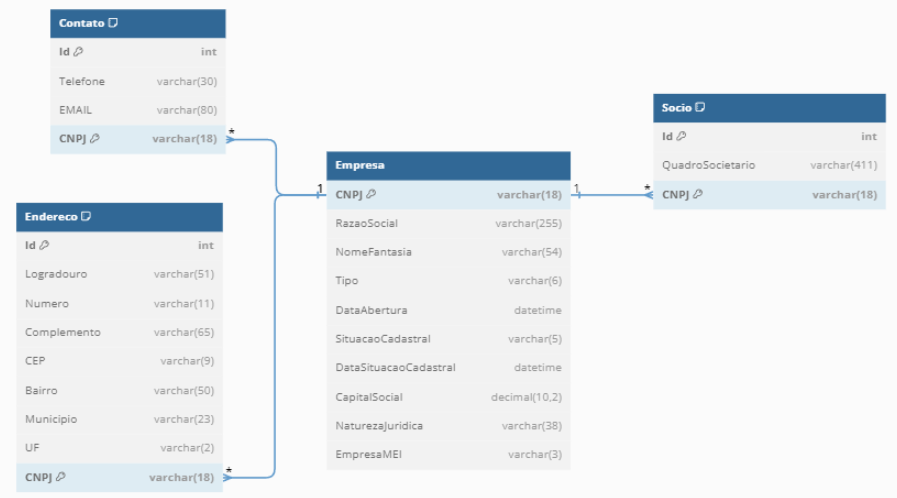
\includegraphics[width=\textwidth]{modelo_latex/figs/modelagem_dados.png}
    \caption{Modelagem de entidades e relacionamentos do banco de dados}
    \label{fig:diagrama_er}
\end{figure}

\subsection{Carga dos dados}

Com os dados modelados e o banco de dados criado, é necessário realizar a carga dos dados. Considerando que a carga dos dados só deve ser executada quando há dados para processar e que assim que a carga for realizada, sua função é finalizada, foi escolhido o serviço AWS Lambda. assim como na etapa de extração dos dados, o Lambda atende a necessidade da solução e apresenta o menor custo possível. A carga será realizada utilizando a linguagem Python e a biblioteca pymysql. Diferente da etapa de extração, o acionamento dessa tarefa é realizada por uma ação e não por agendamento periódico. Isso quer dizer que, sempre que os dados estiverem disponíveis, ele realizará a carga dos dados.

Visando uma melhor manutenção dos dados extraídos, foi sugerido um método de carga dos dados que permitia uma cópia dos dados inseridos no formato CSV. Dessa forma, caso houvesse algum problema com o banco de dados, a informação não seria perdida. Para isso, foi escolhido o serviço AWS S3. O S3 é um serviço de armazenamento de objetos que oferece escalabilidade, disponibilidade de dados, segurança e desempenho líderes do setor \cite{S3}. O S3 permite a criação de buckets, que são repositórios para armazenar arquivos e pastas. Com isso, é possível criar um bucket para armazenar os arquivos CSV gerados pelo processo de carga dos dados.

Com os dados disponibilizados no banco de dados, é necessário disponibilizar esses dados para os times de prospecção do cliente e análise de dados. Para isso, foi escolhido o serviço AWS RDS. Este serviço permite a criação de um banco de dados relacional, que pode ser acessado por qualquer ferramenta de análise de dados. Para esse projeto, foi escolhido o banco de dados Mysql, que é um banco de dados relacional de código aberto, com uma forte ênfase em extensibilidade e conformidade com padrões \cite{MySQL}. O Mysql amplamente utilizado no mercado, o que permite a fácil integração com ferramentas de análise de dados, como por exemplo o PowerBi, que é a ferramenta utilizada pela empresa para a construção dos painéis de análise de dados.

Levando todas essas definições em consideração, a arquitetura proposta para a solução é apresentada na figura \ref{fig:arquitetura_aws}.

\begin{figure}[H]
    \centering
    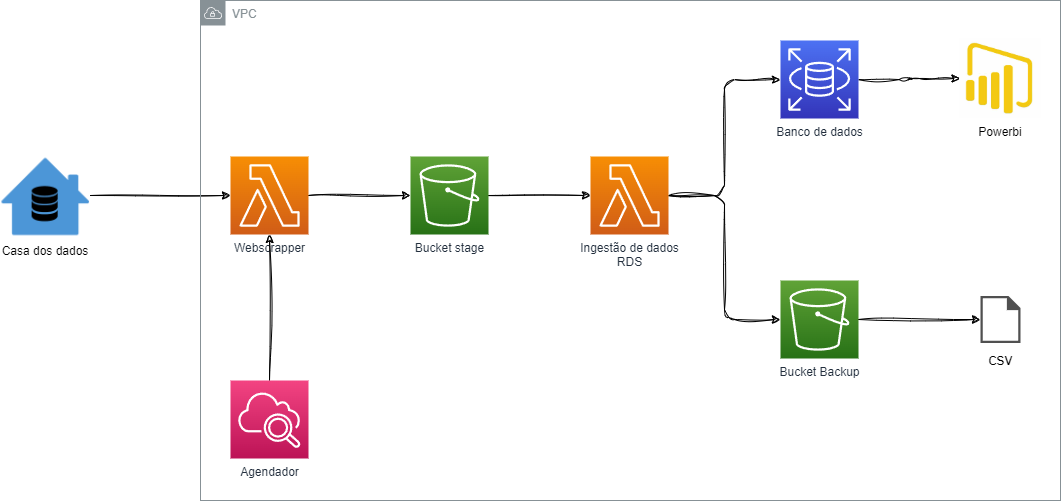
\includegraphics[width=\textwidth]{modelo_latex/figs/arquitetura_aws.png}
    \caption{Arquitetura proposta para a solução}
    \label{fig:arquitetura_aws}
\end{figure}


\section{implementação da solução}

Com a arquitetura definida, é possível realizar o desenvolvimento passo a passo da solução. O primeiro passo é a criação de um repositório no git para o versionamento do código. Para esse projeto, foi escolhido a plataforma Github, pela familiaridade e praticidade de uso. O git permite um desenvolvimento seguro, pois é possível realizar o versionamento e teste de novas características nos algoritmos sem comprometer o código como um todo, sendo possível realizar o rollback caso necessário. Além disso, o git permite a criação de branches, que são ramificações do código principal, permitindo mais clareza no desenvolvimento e aplicando a metodologia de gitflow.

Criado o repositório, foi possível iniciar o desenvolvimento dos algoritmos que serão utilizados na solução.
Para o desenvolvimento dos algoritmos em python, foi gerado um ambiente virtual do Python, permitindo que as bibliotecas que foram usadas no projeto estejam apenas dentro do projeto, sem interferir nas bibliotecas e versões de outros projetos e do python base da máquina local. Essa é uma boa prática de desenvolvimento quando se tem mais de um projeto em python, pois permite que cada projeto tenha suas próprias dependências e versões.

Para o desenvolvimento e teste de funções, métodos e classe, existe um framework chamado Jupyter Lab. Esse framework permite a criação de notebooks, que são arquivos que permitem a execução de código em blocos, permitindo a execução de testes e validação de entradas e saídas das funções desenvolvidas. Para utilizar esse framework, é necessário instalá-lo no ambiente virtual python que será usado utilizando o gerenciador de bibliotecas pip.

\subsection{Extração dos dados}

Como mencionado anteriormente, a extração dos dados será realizada utilizando a biblioteca Scrapy. utilizando o gerenciador de bibliotecas pip, foi feita a instalação no ambiente virtual. feito isso, é necessário realizar uma análise exploratória do site que se deseja extrair as informações.

O site escolhido foi a casa dos dados, pois ele apresenta uma estrutura simples e com poucas informações, o que facilita a extração dos dados. O primeiro passo é identificar qual é a estrutura do site, ou seja, como as informações estão organizadas. Para isso, é utilizado o inspecionar elemento do navegador, que permite a visualização do código fonte do site, bem como o console de rede de comunicação para identificar o tráfico dos protocolos utilizados na comunicação cliente-servidor. Essa análise nos permitirá identificar os elementos e os dicionários de envio e resposta de cada requisição.

O primeiro site que a nossa solução irá interagir será a página de pesquisa avançada do site casadosdados. Esse endpoint permite realizar a busca de CNPJs usando filtros. Para o entendimento de como funciona a comunicação entre o cliente e o servidor, foi realizado uma busca simples, adicionando um filtro de atividade empresarial e de data de abertura. Dessa forma, podemos ver de que forma o site interpreta essas informações e como ele retorna os dados. A figura \ref{fig:inspecao_pagina} apresenta o inspecionar elemento do navegador, onde é possível ver o código fonte do site e o console de rede de comunicação.

\begin{figure}[H]
    \centering
    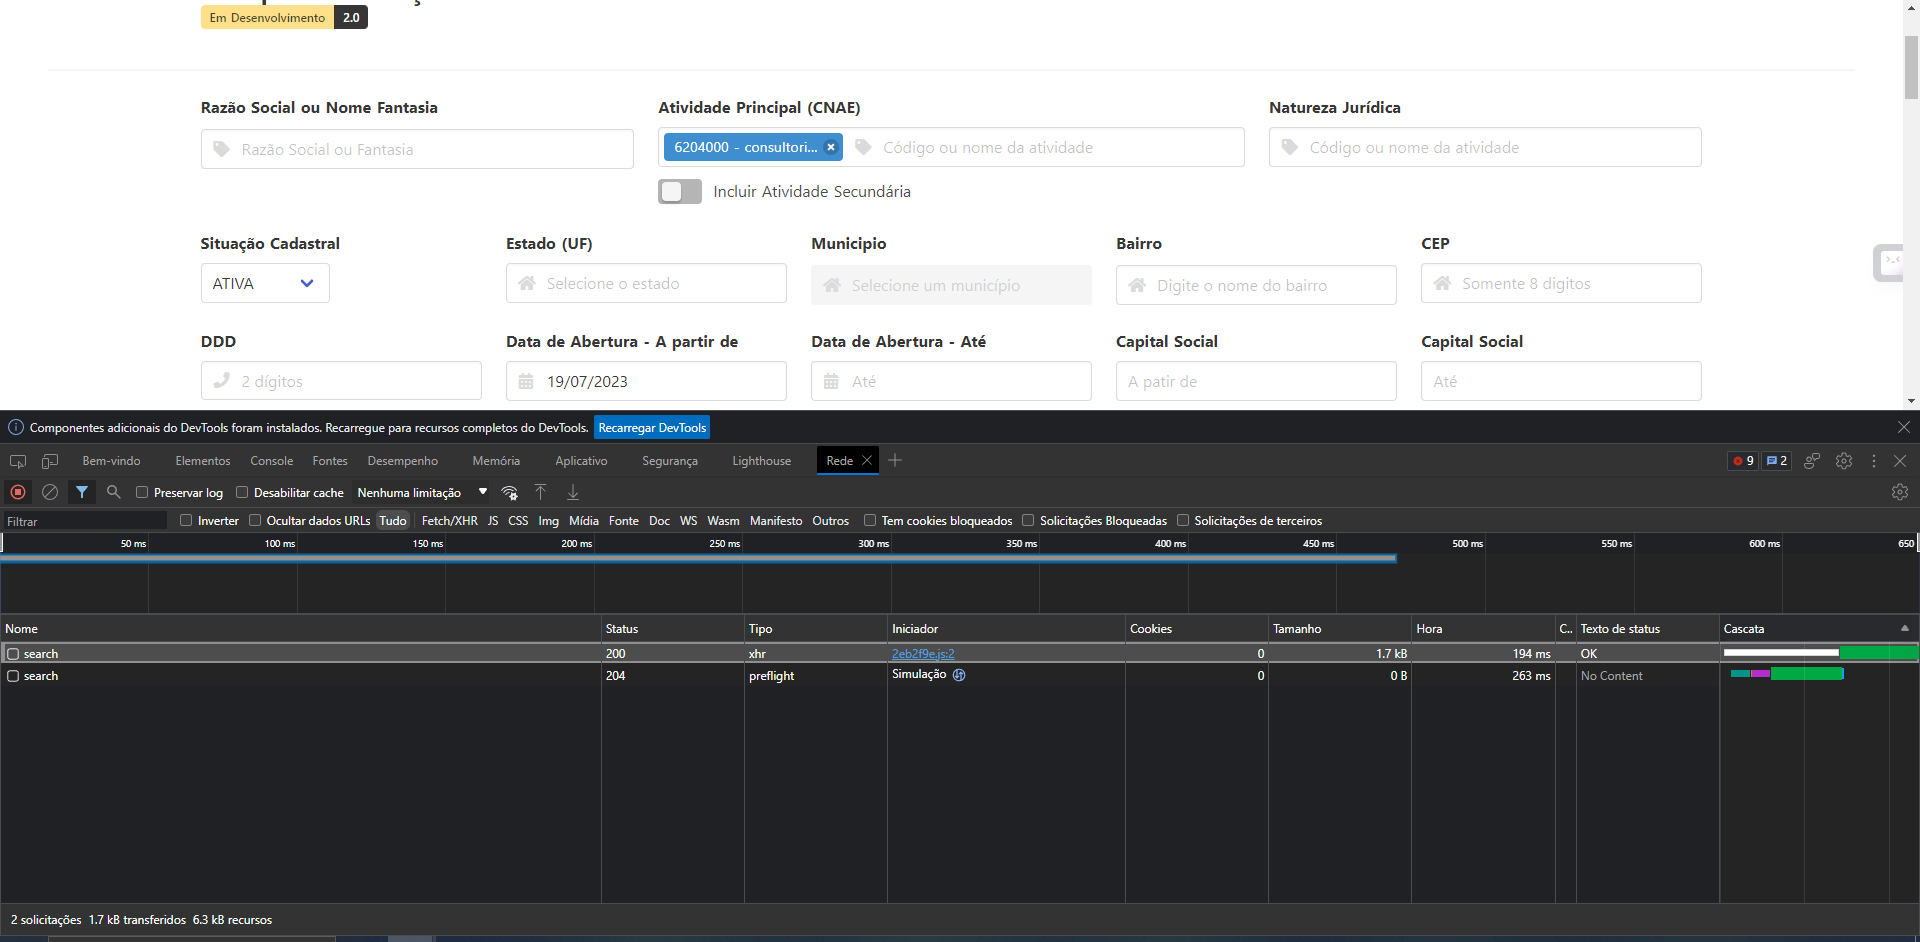
\includegraphics[width=\textwidth]{modelo_latex/figs/inspecao_pagina.png}
    \caption{Inspecionar elemento do navegador}
    \label{fig:inspecao_pagina}

\end{figure}

Ao analisar o tráfego de requisições, foi possível identificar que o site realiza uma requisição POST para o endpoint https://casadosdados.com.br/api/cnpj/search, enviando um dicionário com os filtros de busca.

Com essa informação, é possível construir uma consulta a API, passando os parâmetros desejados e obter a resposta da API, sem a necessidade da construção de um webscrapper propriamente dito, pois a API já retorna os dados em formato json, que é um formato de fácil manipulação e conversão para outros formatos.

Primeiramente, é necessário o entendimento da comunicação com a API para que retorne os resultados esperados. Foi identificado que o protocolo de comunicação é um método POST e possui um header, contendo as informações dos filtros que podem ser aplicados a consulta.
O header de uma consulta a API deve ser apresentado no formato json:

\begin{lstlisting}[language=json]
    {"query":{"termo":[],"atividade_principal":
    ["6204000"],"natureza_juridica":[],"uf":
    [],"municipio":[],"bairro":
    [],"situacao_cadastral":"ATIVA","cep":[],"ddd":
    []},"range_query":{"data_abertura":
    {"lte":null,"gte":"2023-10-02"},"capital_social":
    {"lte":null,"gte":null}},"extras":
    {"somente_mei":false,"excluir_mei":false,"com_email":
    false,"incluir_atividade_secundaria":false,"com_conta
    to_telefonico":false,"somente_fixo":false,"somente_ce
    lular":false,"somente_matriz":false,"somente_filial":
    false},"page":1}
    \end{lstlisting}
    

Com essas informações construídas em formato json e utilizando a biblioteca requests do python, é possível realizar a consulta a API e obter os resultados esperados. A figura \ref{fig:request_response} apresenta a requisição e a resposta do site.

\begin{figure}[H]
    \centering
    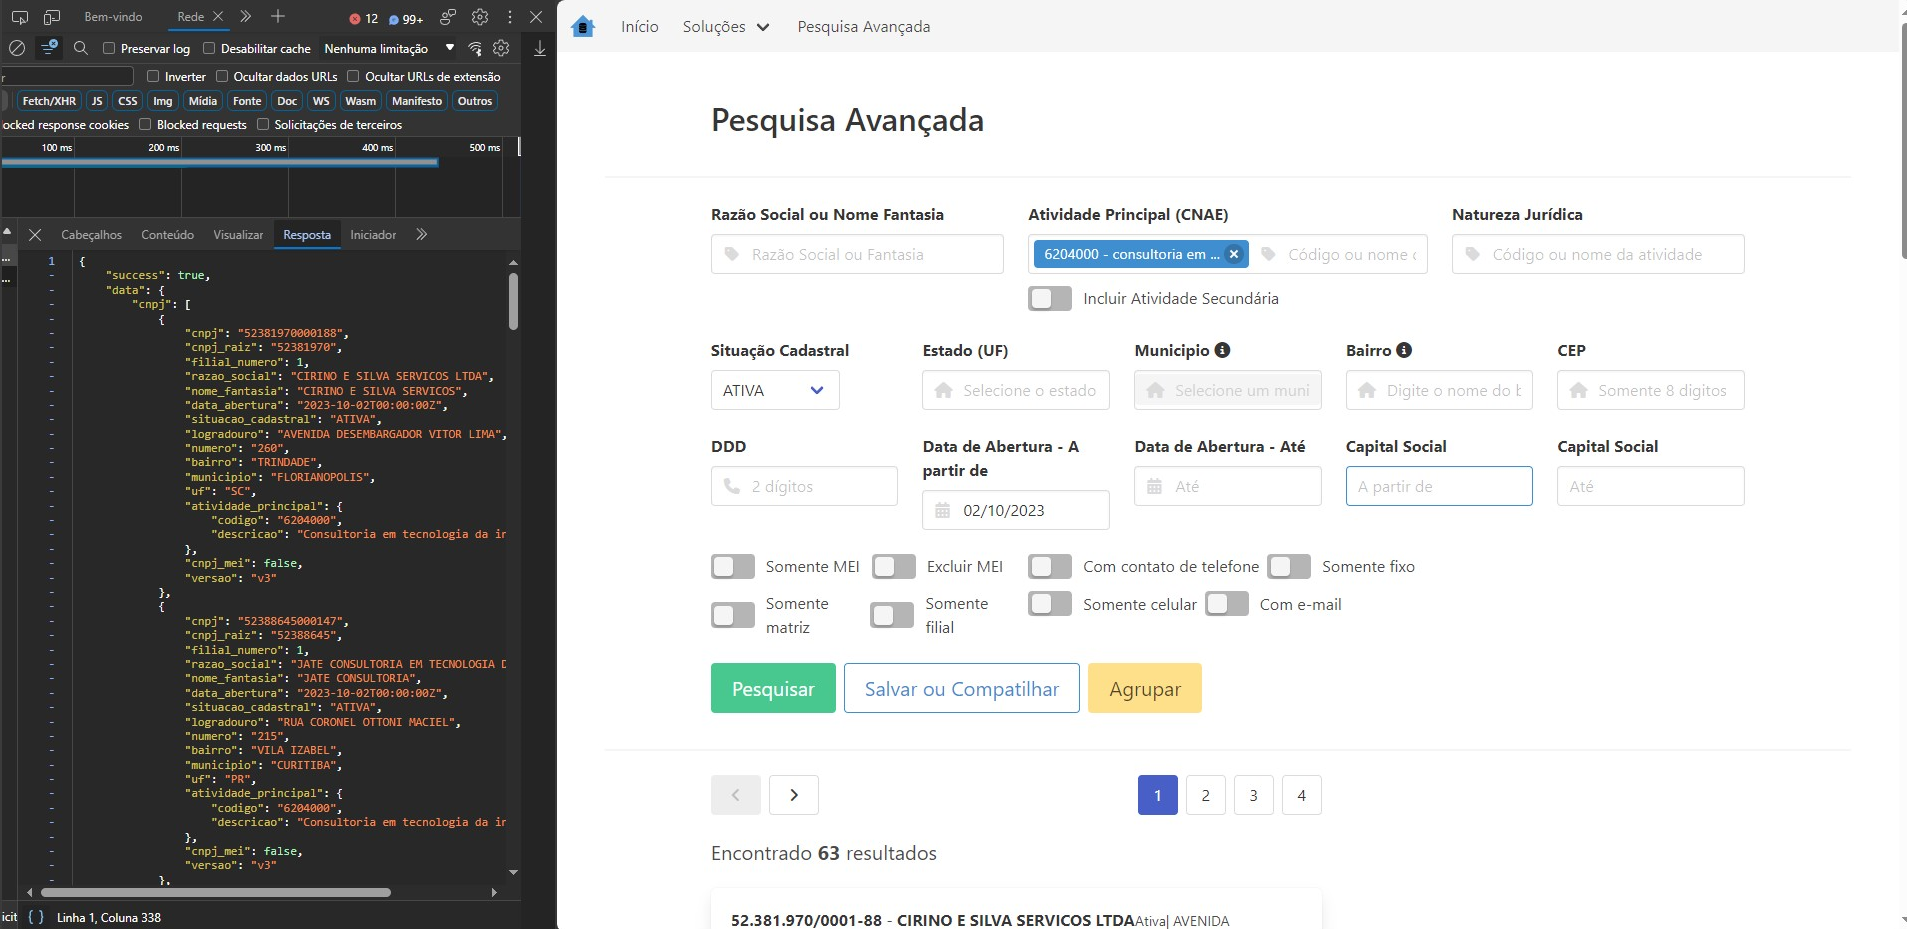
\includegraphics[width=\textwidth]{modelo_latex/figs/response_request.png}
    \caption{Inspecionar elemento do navegador}
    \label{fig:request_response}
\end{figure}

Como foi definido na nossa arquitetura inicial, a extração das informações ocorerrão 1 vez ao dia, identificando todos os CNPJs que foram abertos naquele dia. Para isso, foi definido uma lógica que identifica o dia atual e realiza a consulta a API, passando o dia atual como parâmetro de data de abertura. Também foi notado que a consulta a API retorna 20 resultados por página e possui um parâmetro que indica a página dos dados de resposta. Por exemplo, caso hajam 63 resultados na consulta da API, apenas os 20 primeiros irão ser apresentados na página 1, os próximos 20 serão apresentados na página 2 e assim por diante. Com isso, é necessário construir headers para que todas as páginas sejam extraídas. Para isso, foi construído um laço de repetição que realiza a consulta a API, passando o dia atual como parâmetro de data de abertura e o número da página. A cada iteração, as informações são armazenadas em uma lista, que será utilizada para a construção da próxima requisição de dados, buscando outras informações mais específicas acerca de cada empresa.

O post tem como retorno a seguinte estrutura:

\begin{figure}[H]
    \centering
    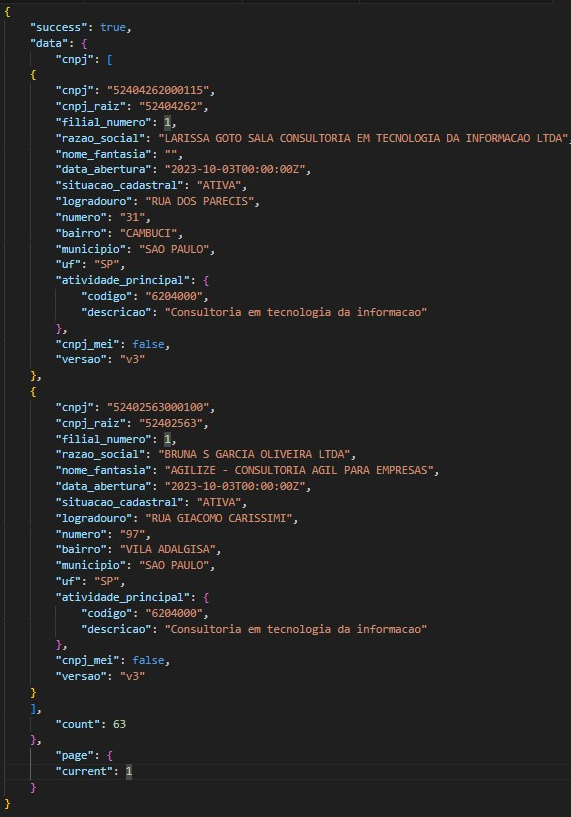
\includegraphics[width=0.7\textwidth]{modelo_latex/figs/json_resposta.png}
    \caption{Resposta do site}
    \label{fig:/json_resposta}
\end{figure}

Essas informações são bem completas, porém não possui todas as informações desejadas. Para isso, é necessário consultar o próximo nível de informações, que é o endpoint para cada uma das empresas, retornando informações mais específicas sobre a empresa. Para isso, é necessário realizar uma consulta a API, passando o CNPJ como parâmetro.

as URLs de cada empresa é construída da seguinte forma:



\url{https://casadosdados.com.br/solucao/cnpj/nome-da-empresa-cnpj}


Para cada informação de empresa extraída da api, é construído uma URL e armazenado em uma lista, contendo todas as URLs que serão utilizadas na segunda etapa do fluxo para a extração das informações mais específicas de cada empresa.

O segundo scrapper é responsável por realizar a raspagem de dados para cada URL que a primeira etapa construiu. o endpoint que será utilizado é o endpoint de detalhes da empresa, que retorna informações mais específicas sobre a empresa, como por exemplo, o capital social, os sócios, o telefone e o e-mail.

A construção da segunda extração de dados exige conhecimento HTML para a utilização da biblioteca Scrapy com mais eficiência. Para encontrar as informações desejadas a serem extraídas, é necessário realizar uma análise exploratória do site para identificar a estrutura do site e como as informações estão organizadas. Para isso, é utilizado o inspecionar elemento do navegador, que permite a visualização do código fonte do site, bem como o console de rede de comunicação para identificar os elementos e os dicionários de envio e resposta de cada requisição.

Através da análise de elementos do site, foi possível identificar que as informações estão organizadas em uma tabela, onde cada linha representa uma informação e cada coluna representa um atributo dessa informação. Para a extração dessas informações, é necessário identificar o elemento que contém a tabela e os elementos que contém as linhas e colunas da tabela. Para isso, é utilizado o inspecionar elemento do navegador, que permite a visualização do código fonte do site, bem como o console de rede de comunicação para identificar os elementos e os dicionários de envio e resposta de cada requisição.

\begin{figure}[H]
    \centering
    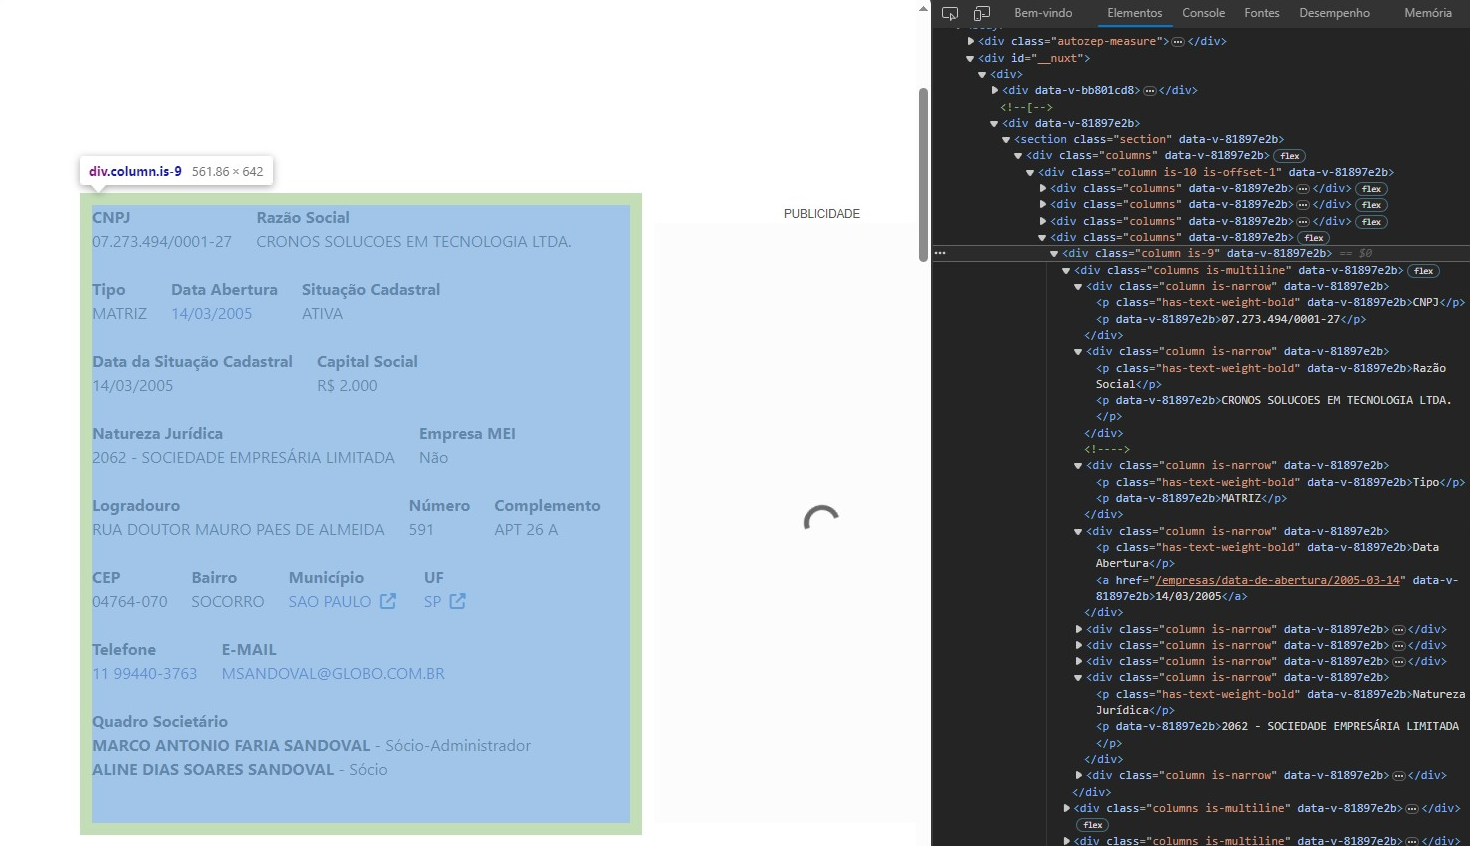
\includegraphics[width=\textwidth]{modelo_latex/figs/investigacao_pagina.png}
    \caption{Análise exploratória da página}
    \label{fig:investigacao_pagina}
\end{figure}

Essa análise permite construir o algoritmo de extração dos dados. A biblioteca utilizada para essa etapa será a scrapy, pois ela permite a construção de webscrappers de forma mais eficiente e rápida. Essa segunda etapa do fluxo da solução receberá a lista de URLs de empresas construída pela etapa anterior e irá realizar a extração dos dados, salvando em um arquivo CSV. Foi necessário levar em consideração alguns tratamentos e validações para que a extração dos dados ocorresse de forma correta. Por exemplo, caso a empresa não possua um e-mail cadastrado ou quadro de sócios, o algoritmo deverá retornar uma string indicando os casos citados. O CSV será salvo em um Bucket-s3, com o objetivo de se manter um histórico de arquivos extraídos, caso haja algum problema com o banco de dados.

\subsection{Ingestão dos dados}

A primeira etapa do fluxo da solução foi responsável pela raspagem de dados e a criação de um arquivo CSV, disponibilizada em um bucket-s3. Com o arquivo CSV disponibilizado, É necessário a ingestão dos dados em um banco de dados relacional para que seja possível realizar a integração e atualização automática dos painéis e relatórios do time de análise de dados. A etapa Ingestão de dados RDS ilustrada na arquitetura \ref{fig:arquitetura_aws} consiste nas seguintes etapas:

\begin{figure}[H]
    \centering
    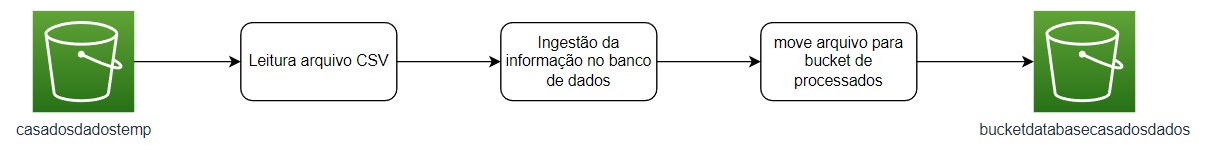
\includegraphics[width=\textwidth]{modelo_latex/figs/arquitetura_ingest.png}
    \caption{Arquitetura da solução de ingestão}
    \label{fig:arquitetura_ingest}
\end{figure}

\begin{itemize}
    \item Extração dos dados do bucket-s3: Realiza a leitura do arquivo CSV disponibilizado no bucket-s3;
    \item Ingestão da informação no banco de dados: realiza as procedures para a ingestão dos dados na tabelas;
    \item move arquivo bucket de processados: Move o arquivo do bucket temporário para o bucket de backup, contendo outros arquivos já processados.
\end{itemize}


Nesse ponto da solução, todos os dados já estão disponíveis de forma organizada e estruturada no banco de dados para os times. Agora os times de análise e prospecção do cliente podem realizar a consulta dos dados para a construção dos painéis. Para o time de prospecção, a disponibilização do arquivo CSV datado com o dia de sua geração é o suficiente para que eles possam entrar em contato com o cliente.

\subsection{Painel de análise de dados}

Para essa etapa, foi escolhida a ferramenta PowerBI, pois já é uma ferramenta utilizada na empresa e que os analistas tem maior familiaridade.
Para que os dados sejam disponibilizados para o PowerBI, é necessário realizar a conexão com o banco de dados. Para fins de exemplo, foi construído o seguinte painel:

\begin{figure}[H]
    \centering
    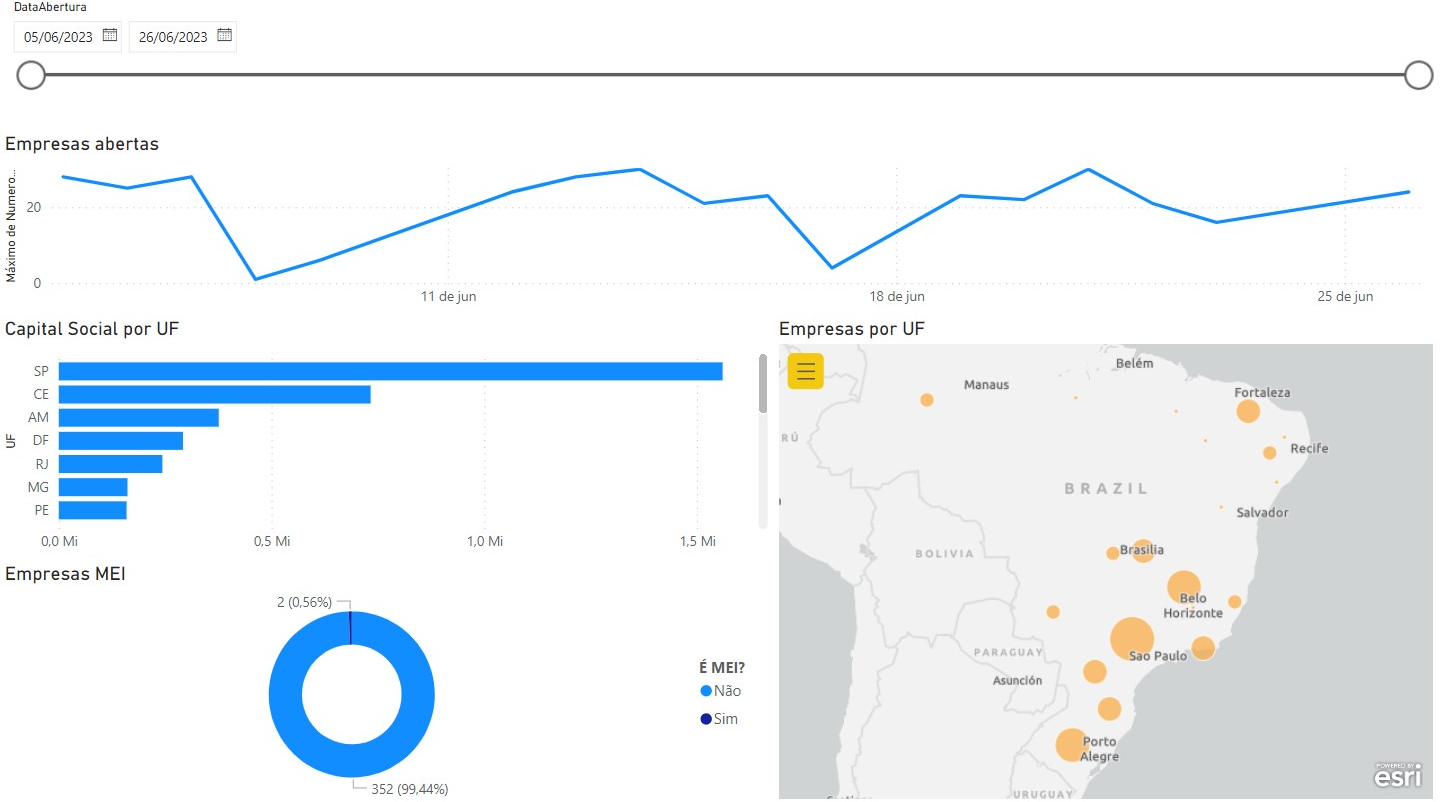
\includegraphics[width=\textwidth]{modelo_latex/figs/dashboard.png}
    \caption{Painel para análise das distribuições de empresas}
    \label{fig:dashboard}
\end{figure}

O painél permite os filtros interativos entre seus componentes, sendo possível realizar filtros por data, por UF e por capital social.

\subsection{devOPS}
